\documentclass{article}
\usepackage{latexsym}
\usepackage{amsmath}
\usepackage{amssymb}
\usepackage{epsfig}
\usepackage{caption}
% \usepackage{psfig}
%\usepackage{epic}
%\usepackage{eepic}
\usepackage{colordvi}
%\usepackage{wrapfig}  
\usepackage{afterpage}
%\usepackage{placeins}
\usepackage{graphics,color}
\usepackage{graphicx}
\usepackage{hyperref}
\usepackage{placeins}
\usepackage{longtable}
\usepackage{color}      % Need the color package
\usepackage{epsfig}
\usepackage{subfiles}
\usepackage[style=nature]{biblatex}
\usepackage{float}
\usepackage{lineno}

\newcommand{\E}{\mathrm{E}}
\newcommand{\Var}{\mathrm{Var}}
\newcommand{\Cov}{\mathrm{Cov}}
\newcommand{\cherry}[1]{\ensuremath{\langle #1 \rangle}}
\newcommand{\eopf}{\framebox[6.5pt]{} \vspace{0.2in}}

%\def\l{{\lambda }}
\def\e{{\varepsilon}}
\def\a{{\alpha }}
\def\S{{\Sigma }}
\def\s{{\sigma }}
\def\M{{\mathcal M}}
\def\X{{\mathcal X }}

\bibliography{EPM-ModeratorsOfAging}

\begin{document}   

\large{\bf{The Epigenetic Pacemaker is a more sensitive tool than penalized regression for 
           identifying moderators of epigenetic aging}}\\ \\
\noindent{\small Colin Farrell$^{1}$, Kalsuda Lapborisuth$^{1}$, Chanyue Hu$^{1}$, Kyle Pu$^{1}$, 
                 Sagi Snir$^{2}$,\\ and Matteo Pellegrini$^{1,3}$\\ \\
\noindent{\footnotesize 
$^1$Dept. of Molecular, Cell and Developmental Biology; \\ University of
California, Los Angeles, CA 90095, USA;;\\
\noindent
$^2$Dept. of Evolutionary Biology, University of  Haifa, Israel;\\
$^3$Corresponding Author, matteop@mcdb.ucla.edu
}

\begin{linenumbers}
\begin{center}\rule{0.9\linewidth}{0.5pt}\end{center}

Epigenetic clocks, DNA methylation based chronological age prediction models, are commonly employed to study age 
related biology. The error between the predicted and observed age is often interpreted as a form of biological 
age acceleration and many studies have measured the impact of environmental and other factors on epigenetic age. 
Epigenetic clocks are fit using approaches that minimize the error between the predicted and observed chronological 
age and as a result they reduce  the impact of factors that may moderate the relationship between actual and 
epigenetic age. Here we compare the standard methods used to construct epigenetic clocks to an evolutionary 
framework of epigenetic aging, the epigenetic pacemaker (EPM) that directly models DNA methylation as a 
function of a time dependent epigenetic state. We show that the EPM is more sensitive than epigenetic clocks for 
the detection of factors that moderate the relationship between actual age and epigenetic state (oe epigenetic age). 
Specifically, we show that the EPM is more sensitive at detecting sex and cell type effects in a large aggregate 
dataset and in an example case study is more sensitive sensitive at detecting age related methylation changes 
associated with polybrominated biphenyl exposure.  Thus we find that the pacemaker provides a more robust 
framework for the study of factors that impact epigenetic age acceleration than traditional clocks based on 
linear regression models.

\begin{center}\rule{0.9\linewidth}{0.5pt}\end{center}
\section{Introduction}

Epigenetic clocks, accurate age prediction models made using DNA methylation, are promising tools for the 
study of aging and age related biology.  Beyond predicting the age of an individual to within a couple of 
years, multiple studies have shown that the difference between the observed and expected epigenetic age 
can be interpreted as a measure of biological age acceleration \cite{Horvath2018-ia}.  Age acceleration 
observed using the first generation of epigenetic clocks \cite{Horvath2013-sk,Hannum2013-um} has been 
associated with a variety of health outcomes including mortality risk\cite{Marioni2015-sn,Perna2016-pi}, 
cancer risk \cite{Dugue2018-ad}, cardiovascular disease\cite{Huang2019-hf} and other negative health 
outcomes\cite{Armstrong2017-vg,Horvath2015-wm,Horvath2014-nx}. However, as epigenetic clocks become more 
accurate, epigenetic age acceleration is no longer associated with mortality \cite{Zhang2019-br}. 
    
Epigenetic clocks are generally trained using a regularized regression model. Given an elastic net model of the 
form $y = \beta X$ the goal of penalized regression is to maximize the likelihood by reducing the prediction error 
of the model, $L(\lambda_1, \lambda_2, \beta) = |y -X\beta|^2+\lambda_2|\beta|^2+|\lambda_1\beta|$. In the case 
of epigenetic clocks, the likelihood is maximized by minimizing the difference between the observed and predicted 
age subject to the elastic net penalty,$\lambda_1$ and $\lambda_2$. . Methylation sites that increase modeled error 
but contain biologically meaningful information may be discarded during model fitting. This problem is magnified in 
the case of epigenetic clocks where the relationship between methylation and time is nonlinear\cite{Snir2019-ii}. 

An alternative and complementary approach to studying epigenetic aging is to model how methylation changes for a 
predetermined collection of sites with respect to time. To this end, we have developed the epigenetic pacemaker 
(EPM) \cite{Snir2016-dv,Farrell2020-ri} to model methylation changes with age. Given $j$ individuals and $i$ 
methylation sites, under the EPM an individual methylation site can be modeled as 
$\hat{m}_{ij} = m^0_i + r_is_j + \epsilon _{ij}$ where $\hat{m}_{ij}$ is the observed methylation value, 
$m^0_i$ is the initial methylation value, $r_i$ is the rate of change, $s_j$ is the epigenetic state, and 
$\epsilon _{ij}$ is a normally distributed error term. The $r_i$ and $m^0_i$ are characteristic of the sites 
across all individuals and the epigenetic state of an individual $s_j$ is set using information from all modeled 
sites. Given an input matrix $\hat M=[\hat  m_{i,j}]$ the EPM utilizes a fast conditional expectation maximization 
algorithm to find the optimal values of $m^0_i$, $r_i$, and $s_j$ to minimize the error between the observed 
and predicted methylation values across a set of sites. This is accomplished by first fitting a linear model 
per site using age as the initial $s_j$. The $s_j$ of the modeled samples is then updated to minimize the error 
between the observed and predicted methylation values. This process is performed iteratively until the reduction 
in error is below a specified threshold or the maximum number of iterations is reached. Under the EPM, the epigenetic 
state has a linear relationship with the modeled methylation data, but not necessarily with chronological age. This 
allows for nonlinear relationships between time and methylation to be modeled without prior knowledge of the underlying 
form. Every modeled methylation site has a characteristic $m^0_i$ and $r_i$ that describes the site in relation to 
other modeled sites and the output epigenetic states. In the current work, we ask whether the EPM formalism can be 
utilized for the identification of moderators that impact the association between age and epigenetic state 
(i.e factors that accelerate or decelerate the changes in epigenetic states with time).  To this end we extend the 
EPM model to simulate methylation matrices associated with age and age accelerating phenotypes. We then evaluate the 
ability of regularized regression and EPM models to detect age acceleration traits that have linear and nonlinear 
associations with age.  Utilizing a large aggregate dataset we validate the simulation results and in one 
illustrative example further assess the ability of both approaches to detect age related methylation 
changes associated with PBB exposure.

\section{Results}

\subsection{Simulation of Trait Associated Methylation Matrices}

Under the EPM the epigenetic state for individual $j$, $S_j$, can be interpreted as a form of biological age that
represents a weighted sum of aging associated phenotypes 
$S_j = \sum^n_{k=1} \alpha_{1} p_{1,j} + ... + \alpha_{k} p_{k,j}$. Under this model $\alpha_{k}$ is the weight for 
phenotype $k$ and $p_{k,j}$ is the value of phenotype $k$.  Phenotypes may contribute to increased or decreased 
aging respectively and when considered as a whole contribute to the overall aging rate observed for an individual.

As shown in our previous work\cite{Snir2019-ii}, the relationship between $p_{k,j}$ and time is not necessarily 
linear. When simulating age associated phenotypes, each phenotype can be represented as 
$p_{k,j} = Age_j^{\gamma_{k}} q_{k,j}$, where $\gamma_{k}$ is a phenotype specific parameter shared among all 
individuals and $q_{j,k}$ represents the magnitude of exposure for a simulated trait and is personal to an 
individual. The observed phenotype is modeled as an interaction between age and an exposure of varying magnitude 
among individuals. This formulation is flexible as non-age dependent traits can be easily simulated by setting 
$\gamma_{k}=0, p_{k,j} = q_{k,j} = Age_j^{0}q_{k,j}$.  Individual sites can be described as a linear model where 
$\hat{m_{i,j}} = m^0_i + r_i P_{i,j} + \epsilon_{i,j}$. $P_{i,j}$ is a weighted sum of phenotypes influencing the 
methylation status of an individual site, $P_{i,j} = \sum^n_{k=1} \upsilon_{1} p_{1,j} + ... + \upsilon_{k} p_{k,j}$. 

To assess the sensitivity of the EPM and penalized regression approaches at detecting moderator of epigenetic aging we 
simulated a methylation matrix containing linear and nonlinear age associated traits of form 
$p_{k,j} = Age_j^{\mathcal{N}(0.5, 0.01)} q_{k,j}$ and $p_{k,j} = Age_j^{\mathcal{N}(1, 0.01)} q_{k,j}$. The 
trait $\gamma$ parameter was generated by sampling from a normal distribution $\mathcal{N}(0.5, 0.01)$ to generate 
traits with varying relationships with time (Figure 1). Samples were simulated by assigning an age from a uniform 
distribution, $\mathcal{U}(0,100)$ and setting sample health  by sampling from a normal distribution. Sample health 
is a sample specific metric that influences the magnitude and direction of the simulated age accelerating trait. 
Simulated traits included a binary phenotype  $(P=0.5)$, continuous phenotypes influenced by only age, or by age and 
sample health (Table 1). The effect, $q$, of a binary trait was varied from 0.995 to 1.0 over 5 equally spaced 
intervals. Given a binary trait form of $p_{k,j} = Age_j^{0.5} q_{k,j}$ a 0.001 decrease in $q$ corresponds to a 
1 percent decrease in epigenetic state by age 100 relative to samples not assigned the binary trait. Within each 
interval the standard deviation of the sample health sampling distribution was varied from 0.0 to 0.01 over 5 
equally spaced intervals. The simulation was repeated 50 times for each binary, continuous trait combination with 
500 simulated samples within each simulation. Additionally, at a binary $q$ of 0.995 the range of continuous traits 
was expanded over a broader range to assess the model sensitivity for detecting the continuous trait. Five methylation 
sites for all continuous traits were then simulated and 50 methylation sites for the binary trait. An additional 50 
sites were simulated that were equally influenced by a mixture of four continuous traits and the simulated  binary 
trait. The resulting simulation matrix contains 450 methylation sites. 

Given a simulation dataset, the samples were split randomly in half for model training and testing. EPM and penalized 
regression models were fit for each simulation training set and epigenetic state and age predictions were made for the 
testing set. e then fit a regression model where the epigenetic age or state is dependent on the age, square-root of 
the age, the health status, and binary trait status of the sample ($S_j  = Age + \sqrt{Age} + health_j + binary_j$). 
The square-root of the age is included in the regression model to account for the nonlinear relationship between the 
simulated age and methylation data. 

As the exposure size of the binary trait is decreased from 1.00 to 0.995 the ability to detect the influence of the 
trait on the epigenetic state and age is improved (Figure 2A and B). At an effect size of 0.995 the estimated effect 
of the binary trait on the epigenetic state is significant ($\mu =0.035, \sigma=0.089$) while the effect on the 
epigenetic age it is not ($\mu=0.269, \sigma=0.282$). At an exposure size of 1.0, where the simulated binary trait 
has no effect, the distribution of p values forEPM and linear models is randomly distributed. The ability to observe 
the health effect of the simulated continuous traits improves in both the linear and EPM models as the standard 
deviation of the sample health sampling distribution is increased (Figure 2 C and D). At an exposure size of 0.002 
and 0.0025 the average EPM model is significant ($\mu=0.0194, \sigma=0.0436$) while the average linear model is not 
($\mu=0.0607, \sigma=0.128$). At a continuous trait standard deviation above 0.005 both models produce significant 
results. 

\subsection{Universal Blood EPM and Penalized Regression Models}

We validated the simulation results using a  large aggregate dataset composed of Illumina 450k array 
data\cite{Marabita2018-yi,Ventham2016-qj,Tan2014-ns,Johnson2020-vb,Voisin2015-ch,Soriano-Tarraga2016-tf,
Dabin_undated-pr,Horvath2015-af,Kurushima2019-gc,Zannas2019-bc,Braun2019-gp,Demetriou2013-jx,Tserel2015-qr} 
deposited in the Gene Expression Omnibus\cite{Barrett2012-gu} (GEO). All methylation array datasets were processed 
using a unified pipeline from raw array intensity data (IDAT) files using minfi (Aryee et al., 2014). Sex and blood 
cell type abundance predictions were made for each processed as previously described\cite{Houseman2012-rr,Aryee2014-ky}. 
The aggregate dataset contains 6,251 whole blood tissue samples representing 16 GEO series. 

We trained EPM and penalized regression models using data assembled from four GEO 
series\cite{Johansson2013-of,Liu2013-qo,Butcher2017-nr,Damaso2020-gd}  ($n=1605$) with samples spanning a wide age 
range (0.01 - 94.0 years). The training set was split by predicted sex, within each sex we used stratified sampling by 
age to select 95\% of the samples for model training. The selected samples from each sex were combined 
($n=1524$) and the remaining samples ($n=81$) left out for  model evaluation. Methylation values for all samples were 
quantile normalized by probe type\cite{Horvath2013-sk} using the median site methylation values across all training 
samples for each methylation site.  Principal component analysis (PCA) was performed on the cell type abundance 
estimates using the training data. The trained PCA model was used to predict the cell type PCs for the testing 
and validation datasets. 

We fit a penalized regression model to the training matrix as follows. The normalized training methylation matrix was 
first filtered to remove sites with a variance below 0.001, resulting in a training matrix with 183,114 sites. A 
cross validated ($cv=5$) elastic net model was trained against training sample ages using the filtered methylation 
matrix. The trained model performed well on the training ($R^2=0.981$) and testing ($R^2=0.940$) datasets (S.Figure 2). 

In contrast to penalized regression based approaches, site selection for the EPM model is performed outside of model 
fitting. Methylation sites were selected for model training if the absolute Pearson correlation coefficient between 
methylation values and age was greater than 0.4 ($n=16,880$). A per site regression model was fit using the observed 
methylation value as the dependent variable and age as the explanatory variable. Sites with a mean absolute error 
(MAE) less than 0.025 between the predicted and observed methylation values were retained for further analysis 
($n=7,013$). An EPM model was fit using these sites (Figure 3A). We then sought to identify subsets of sites that 
had functionally similar forms between age and methylation. This was done to filter sites that were associated with 
age by chance and to select clusters of sites with low prediction error. Subsets of sites with similar functional form 
were identified by clustering sites using affinity propagation \cite{Frey2007-mu}) by the euclidean distance between 
the single site regression model residuals. Cross validated EPM and penalized regression models were trained for all 
clusters with greater than ten sites ($n=55$). The cluster EPM models show varying associations between the epigenetic 
state and age relative to the EPM model fit with all sites initially selected by absolute PCC(Figure 3B). Clusters 
with an observed EPM and penalized regression MAE less than 6 ($n=5$) were combined to fit final EPM and penalized 
regression models. This resembles the simulated methylation matrices where sites with differing functional forms are 
modeled collectively. The combined cluster EPM and combined cluster regression model performed well on the training 
and testing datasets (S.Figure 1). 

We evaluated the combined cluster EPM, combined cluster penalized regression, and the full penalized regression models 
against a validation data set consisting of 14 GEO series experiments representing 4,600 whole blood tissue samples. 
Each model accurately predicted the epigenetic state or epigenetic age of the validation samples (Figure 4). We then 
fit an ordinary least squares regression model for every validation experiment individually to predict the observed 
epigenetic age or state using the sample age, the square root of age, cell type PCs, and predicted sex 
($S_j  = Age + \sqrt{Age} + PC1 + PC2 + PC3 + Sex + Intercept$). If the proportion of female samples to the total 
number of samples was greater than 0.7 the sex term was dropped from the regression model. Significant cell type 
PC2 coefficients were observed for all EPM models and the majority of the cluster and full penalized regression 
models (Figure 5A). Significant cell type PC1 and PC3 coefficients were observed for the majority of the EPM models 
but not for the cluster or full penalized regression models. Significant sex effects ($p < 0.0038$) were 
observed for 9, 4, 0 out of 15 models for the EPM, cluster penalized regression, and full penalized regression 
respectively (Figure 5B). 

\subsection{Polybrominated Biphenyls Exposure}

Polybrominated biphenyls (PBB) were widely used throughout the United States in the 1960’s and 1970’s for a variety of 
industrial applications. Widespread PBB exposure occurred in the state of Michigan from the summer of 1973 to later 
spring of 1974 when an industrial PBB mixture was incorrectly substituted for a nutritional supplement used in livestock 
feed\cite{Fries1985-nf}. PBB is biologically stable and has a slow biological half life; individuals exposed during the 
initial 1973 - 1974 incident still have detectable PBB in their blood\cite{Safe1984-sz}. PBB is an endocrine-disrupting 
compound and exposure has been linked to numerous adverse health outcomes in Michigan residents such as thyroid 
dysfunction\cite{Jacobson2017-yi,Curtis2019-mv} and various cancers\cite{Terrell2016-yw,Hoque1998-so}. A study by 
Curtis et al. showed total PBB exposure is associated with altered DNA methylation at CpG sites enriched for an 
association with endocrine-related autoimmune disease \cite{Curtis2019-gz}. Utilizing the publicly available 
Illumina Methylation EPIC array \cite{Pidsley2016-bg}  profiles ($n=679$), that covered a wide age range 
(23 - 88 years), we sought to compare the ability of penalized regression and the EPM to detect epigenetic age 
acceleration associated with PBB exposure. 

Briefly, 50\% of samples ($n=339$) were selected for model training using stratified cross validation by age. A 
cross validated elastic net model was trained using all methylation sites with a site variance above 0.001, 
($n=529,703$). The trained model performed well on the training and testing datasets 
($R^2 = 1.00, R^2 = 0.740, S.Figure 2 A-B$). EPM sites were selected and models fit as described with the universal 
blood EPM. Four EPM clusters ($MAE < 6$) were merged for a combined EPM model built using 413 CpG sites. The 
combined EPM model performed well in training and testing datasets ($R^2 = 0.794, R^2 = 0.812, S.Figure 2 C-D$). 
Epigenetic age and epigenetic state predictions were then made for the testing samples using the penalized 
regression and EPM models. 

We then fit an OLS regression model to predict the epigenetic age or state dependent on  PBB-153 exposure, h age, the 
square root of age, cell type PCs, and predicted sex 
($S_j  = Age + \sqrt{Age} + PC1 + PC2 + PC3 + Sex + PBB-153 + Intercept$). PBB-153 exposure was highly significant in 
the EPM regression model ($p=5.9e-10$) but not the penalized regression model ($p=0.141$). 

\section{Discussion}

A long standing question in the field of epigenetics was whether biomarkers could be trained to predict various 
traits using methylation measurements.  The most successful biomarkers to date have been epigenetic clocks that can 
accurately predict the age of an individual based on their methylation pattern. These have been shown to be useful for 
human studies of aging, as well as for animal studies, including mice\cite{Thompson2018-rh} and dogs\cite{Thompson2017-cl}.  
DNA methylation biomarkers are typically constructed using penalized regression approaches.  Given a large enough matrix, 
penalized regression will select sites that minimize the prediction error given a modeled trait. Epigenetic clocks 
are examples of such models.  Beyond predicting actual ages, these models have also been used to measure the influence 
of external factors on the rates of aging, and multiple studies have shown that the resulting age accelerations 
(i.e the differences between actual and predicted ages) are significantly associated with multiple factors such as 
cardiovascular disease\cite{Huang2019-hf} and mortality risk\cite{Marioni2015-sn,Perna2016-pi}.

While epigenetic clocks have proven to be useful they have significant limitations.  Because they are based on linear 
models, it may be difficult to model aging when the underlying methylation changes are non-linear in time.  Moreover, 
epigenetic clocks are prone to over fitting, and while cross validation schemes are often used to construct 
robust clocks, they often do not yield accurate estimates for other datasets.  Finally, epigenetic clocks are not 
very interpretable, and highly degenerate, so that it is difficult to extract biological insights from the weights 
of the models.

To overcome some of these limitations, we have previously developed the epigenetic pacemaker formalism.  In this 
approach, rather than building a model for the age, we construct a model for the observed methylation data that 
depends on age.  The advantage of this approach is that this formalism allows us to identify non-linear associations 
between methylation and age across a lifespan.  Moreover, these models tend to be robust to training as they are fit 
to large methylation matrices rather than age vectors. Finally, the model describes the change in methylation at each 
site with respect to a time dependent epigenetic state, and therefore all parameters of the model are directly 
interpretable as either initial values of methylation or rates of change of methylation.

Depending on the context, epigenetic clocks are both more and less effective than the EPM. The penalized regression 
models provide more accurate age predictions ($R^2=0.875,0.911$) than the EPM model ($R^2=0.821$), and the model 
output can be directly compared to the age of a sample. However, because these models are optimized to reduce the 
error between actual and predicted age, they tend to minimize the effect of extraneous factors on the predicted age.  
As such, epigenetic clocks are not optimal for identifying external factors that moderate the relations between actual 
and predicted age.  By contrast, the EPM models are not optimized to minimize the difference between predicted and 
actual age, but rather try to minimize the difference between observed and modeled methylation values.  As such, they 
retain many of the effects that other factors may have on the association between methylation and epigenetic states.  

In this study we find that while the penalized regression models were more accurate for predicting age, the epigenetic 
state generated by the EPM is significantly impacted by  cell type and sex effects in both simulations and real data. 
We also found that The EPM model generated for individuals exposed to PBB was sensitive to e PBB exposure, which has 
been linked to negative health outcomes, while the penalized regression epigenetic aging model was not. Additionally, 
the sensitivity of the EPM to moderators of epigenetic aging has been supported by two two recent studies  
investigating epigenetic aging in marmots\cite{Pinho2021-gm} and zebras\cite{Larison2021-ts}. In the first of 
these studies, EPM models showed an association between hibernation and slowed epigenetic aging in marmots and 
in the second an increased epigenetic age associated with zebra inbreeding; no such associations were observed with 
penalized regression epigenetic age models. 

Most studies of human epigenetic aging are not motivated by the development of accurate age predictors, since ages 
are nearly always known in studies,  but rather by the discovery of  biological aging moderators. The EPM is a more 
sensitive approach than epigenetic clocks for the detection of factors other than age that influence the epigenome  
and therefore potentially more useful for discovering moderators of biological aging. 

\section{Methods}

\subsection{Simulation}

We implemented the simulation framework as a python package with numpy($\geq$v1.16.3)\cite{Harris2020-yb} and 
scikit-learn(v0.24)\cite{Pedregosa2011-fi} as dependencies. A simulation run generates  a trait-associated methylation
matrix and samples are tied to the simulated  traits. The simulation procedure is implemented as follows:
\begin{itemize}

    \item{Traits are intialized that contain the information about the trait relationship with age and a 
    simulated sample phenotype. Given the structure $p_{k,j} = Age_j^{\gamma_{k}} q_{k,j}$, and $k$ samples 
    and $j$ traits $\gamma$ is characteristic of the trait. When a sample is passed to a trait, a value of $q$ is
    generated for the sample by sampling from a normal distribution with a variance characteristic of the 
    simulation trait. Additionally, each trait can be optionally influenced by a characteristic measure of sample 
    health, $h_j$. Given, a normally distributed trait $\mathcal{N}(\mu,\sigma^{2})$ and a health effect $h_j$, 
    the sampled distribution for individual $j$ is $\mathcal{N}(\mu + h_j,\sigma^{2})$. Continuous and binary 
    traits can be simulated. If a binary trait is simulated, a $q$ other than 1 is assigned at a 
    specified probability.}
     
    \item{Samples are simulated by setting the age by sampling from a uniform distribution over a specified range 
    and by setting a sample health metric $h$ by sampling from a normal distribution centered on zero with a 
    specified variance. Traits passed to a sample simulation object are then set according to the age and 
    health of the sample. Simulated samples retain all the set phenotype information for downstream reference.}

    \item{Methylation sites are simulated by randomly setting the initial methylation value, maximum observable 
    methylation value, the rate of change at the site, and the error observed at each site. Sites are then assigned 
    traits that influence the methylation values at each site.}

    \item{Methylation values are simulated for each site for every individual given the simulated phenotypes with a 
    specified amount of random noise.}
\end{itemize}

\subsection{Simulation EPM and Penalized Regression Models}

Simulation data was randomly split in half into training and testing sets. EPM models were fit using the 
simulated methylation matrix against age. Penalized regression models were fit 
using scikit-learn(v0.24)\cite{Pedregosa2011-fi} ElasticNet (alpha=1, l1\_ratio=0.75, and selection=random). 
All other parameters were set to their default values. Ordinary least squares regression as implemented in 
statsmodels (0.11.1)\cite{Seabold2010-lt} was utilized to describe the epigenetic state or age with the following 
form ($S_j  = Age + \sqrt{Age} + health_j + binary_j$). Full analysis is found in the 
EPMSimulation.ipynb supplementary file.  

\subsection{ Methylation Array Processing}

Metadata for Illumina methylation 450K Beadchip methylation array experiments deposited in the Gene Expression 
Omnibus (GEO) \cite{Barrett2012-gu} with more than 50 samples were parsed using a custom python tool set. Experiments 
that were missing methylation beadchip array intensity data (IDAT) files, made repeated measurements of the same 
samples, utilized cultured cells, or assayed cancerous tissues were excluded from further processing. IDAT files 
were processed using minfi\cite{Aryee2014-ky} (v1.34.0). Sample IDAT files were processed in batches according to 
GEO series and Beadchip  identification. Methylation values within each batch were normal-exponential normalized 
using out-of-band probes\cite{Triche2013-pp}. Blood cell types counts were estimated using a regression calibration 
approach\cite{Houseman2012-rr} and sex predictions were made using the median intensity measurements of the X and Y 
chromosomes as implemented in minfi\cite{Aryee2014-ky}. Whole blood array samples were used for downstream analysis 
if the sample median methylation probe intensity was greater than 10.5 and the difference between the observed and 
expected median unmethylation probe intensity is less than 0.4, where the expected median unmethylated signal is 
described by ($y=0.66x + 3.718$). 

\subsection{Blood EPM and Penalized Regression Models}

Methylation sites with an absolute Pearson correlation coefficient between methylation values and age greater than 
0.40 and 0.45 for the unified whole blood and PBB datasets respectively were initially selected for EPM model 
training. A linear model was generated using numpy polyfit \cite{Harris2020-yb} with age and the independent 
variable and methylation values as the dependent variable. Mean absolute error (MAE) was calculated as the mean 
absolute difference between the observed and predicted meth values according to the site linear models. A vector 
of residuals generated using these models were utilized for clustering by affinity propagation\cite{Frey2007-mu}) 
as implemented in scikit-learn (v0.24)\cite{Pedregosa2011-fi} with a random state of 1 and a cluster preference of 
-2.5. Cross-validated EPM, and penalized regression models for the universal blood analysis,  were trained for all 
clusters containing greater than ten sites. Clusters with an observed EPM and penalized regression MAE less than 6.0 
were combined to fit final EPM and regression models. 

Penalized regression models were fit using scikit-learn(v0.24)\cite{Pedregosa2011-fi} 
ElasticNetCV (cv=5 alpha=1, l1\_ratio=0.75, and selection=random). All other parameters were set to their 
default values. Principal Component Analysis as implemented in scikit-learn was utilized with default parameters 
to perform PCA on training sample cell type abundances. The trained PCA was utilized to calculate cell type PCs 
for the testing and validation samples. Ordinary least squares regression as implemented in statsmodels 
(0.11.1)\cite{Seabold2010-lt} was utilized describe the epigenetic state or age with the following 
form ($S_j  = Age + \sqrt{Age} + Cell Type PC1 + Cell Type PC2 + Cell Type PC3 + Sex + Intercept$). 
Full analysis is found in the EPMUniversalClock.ipynb supplementary file. 

\subsection{Analysis Environment}

Analysis was carried out in a Jupyter\cite{Basu_undated-vq} analysis environment.
 Joblib\cite{Varoquaux2009-al}, SciPy\cite{Virtanen2020-wt}, Matplotlib\cite{Hunter2007-nq}, 
 Seaborn\cite{Waskom2021-gj}, Pandas\cite{McKinney2012-ta} and TQDM\cite{Da_Costa-Luis2019-lr} p
 ackages were utilized during analysis. 

\subsection{Supplementary Information}

Analysis code and notebooks can be found at https://github.com/NuttyLogic/EPM-ModeratorsOfAging.

\end{linenumbers}
\printbibliography



\begin{table}[H]
\caption*{\textbf{Table 1:} Simulated Trait Conditions}  
\begin{tabular}{| p{20mm} | p{15mm} | p{20mm} | p{20mm} | p{20mm} | p{20mm} | p{20mm} |}
\hline
\textbf{Trait Form}&\textbf{Beta}&\textbf{Gamma}&\textbf{Gamma Std. Dev.}&\textbf{Sample Effect}&
\textbf{Age Only}&\textbf{Generated Phenotypes}\\ \hline
Continuous&0.1&$\mathcal{N}(0.5, 0.01)$&0.05&Yes&No&10\\ \hline
Continuous&0.1&$\mathcal{N}(1.0, 0.01)$&0.05&Yes&No&10\\ \hline
Continuous&0.1&$\mathcal{N}(0.5, 0.01)$&0.05&No&Yes&20\\ \hline
Continuous&0.1&$\mathcal{N}(1.0, 0.01)$&0.05&No&Yes&20\\ \hline
Binary ($Pr=0.5$)&0.1&0.5&0&Yes&No&1\\ \hline
\end{tabular}
\end{table}

\begin{center}
    \begin{figure}
    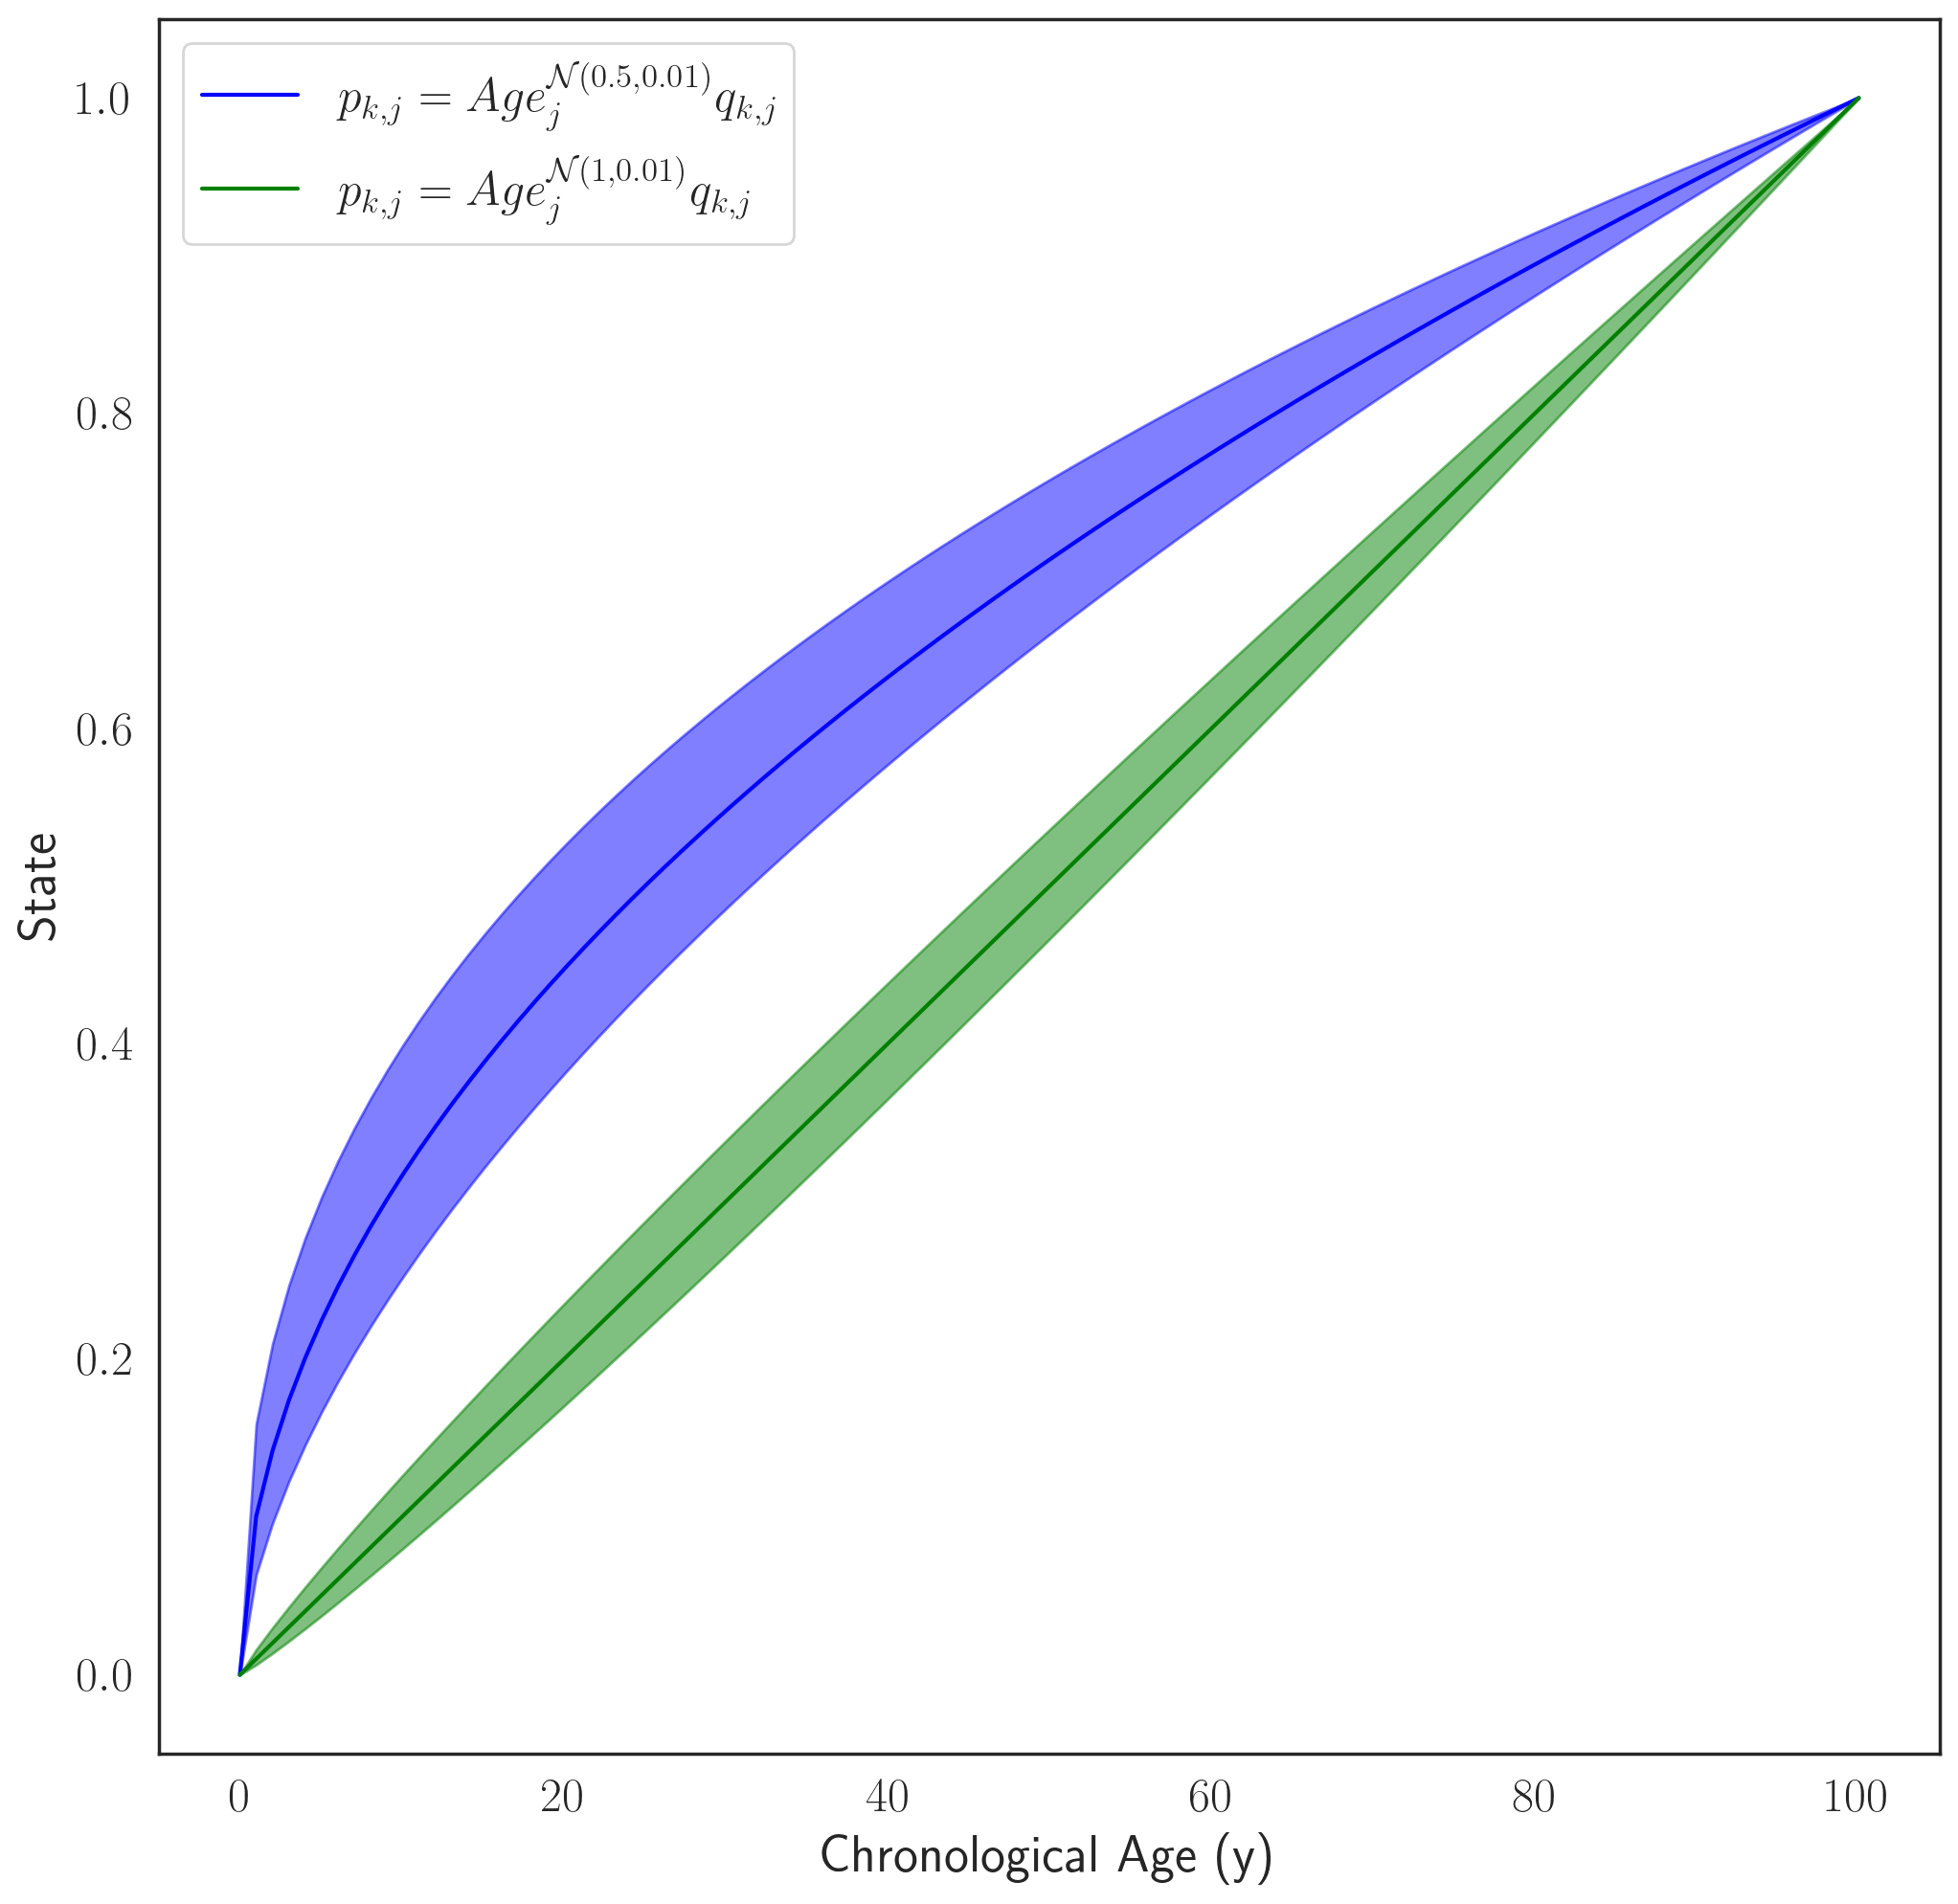
\includegraphics[scale=.4]{Figures/Figure1.png}    
    \footnotesize
    \caption*{\small \textbf{Figure1:} Simulated trait forms where the shaded area represent one 
    standard deviation away from the mean $\gamma$, given $p_{k,j} = Age_j^{\gamma_{k}} q_{k,j}$.}
    \end{figure}
\end{center}

\begin{center}
    \begin{figure}
    \includegraphics[scale=.25]{Figures/Figure2.png}
    \footnotesize
    \caption*{\small \textbf{Figure2:} The distribution binary coefficient p-values for \textbf{A} EPM and \textbf{B} 
    penalized regression models. The distribution of p-values given a simulation health standard 
    deviation for \textbf{C} EPM and \textbf{D} penalized regression models.}
    \end{figure}
\end{center}


\begin{center}
    \begin{figure}
    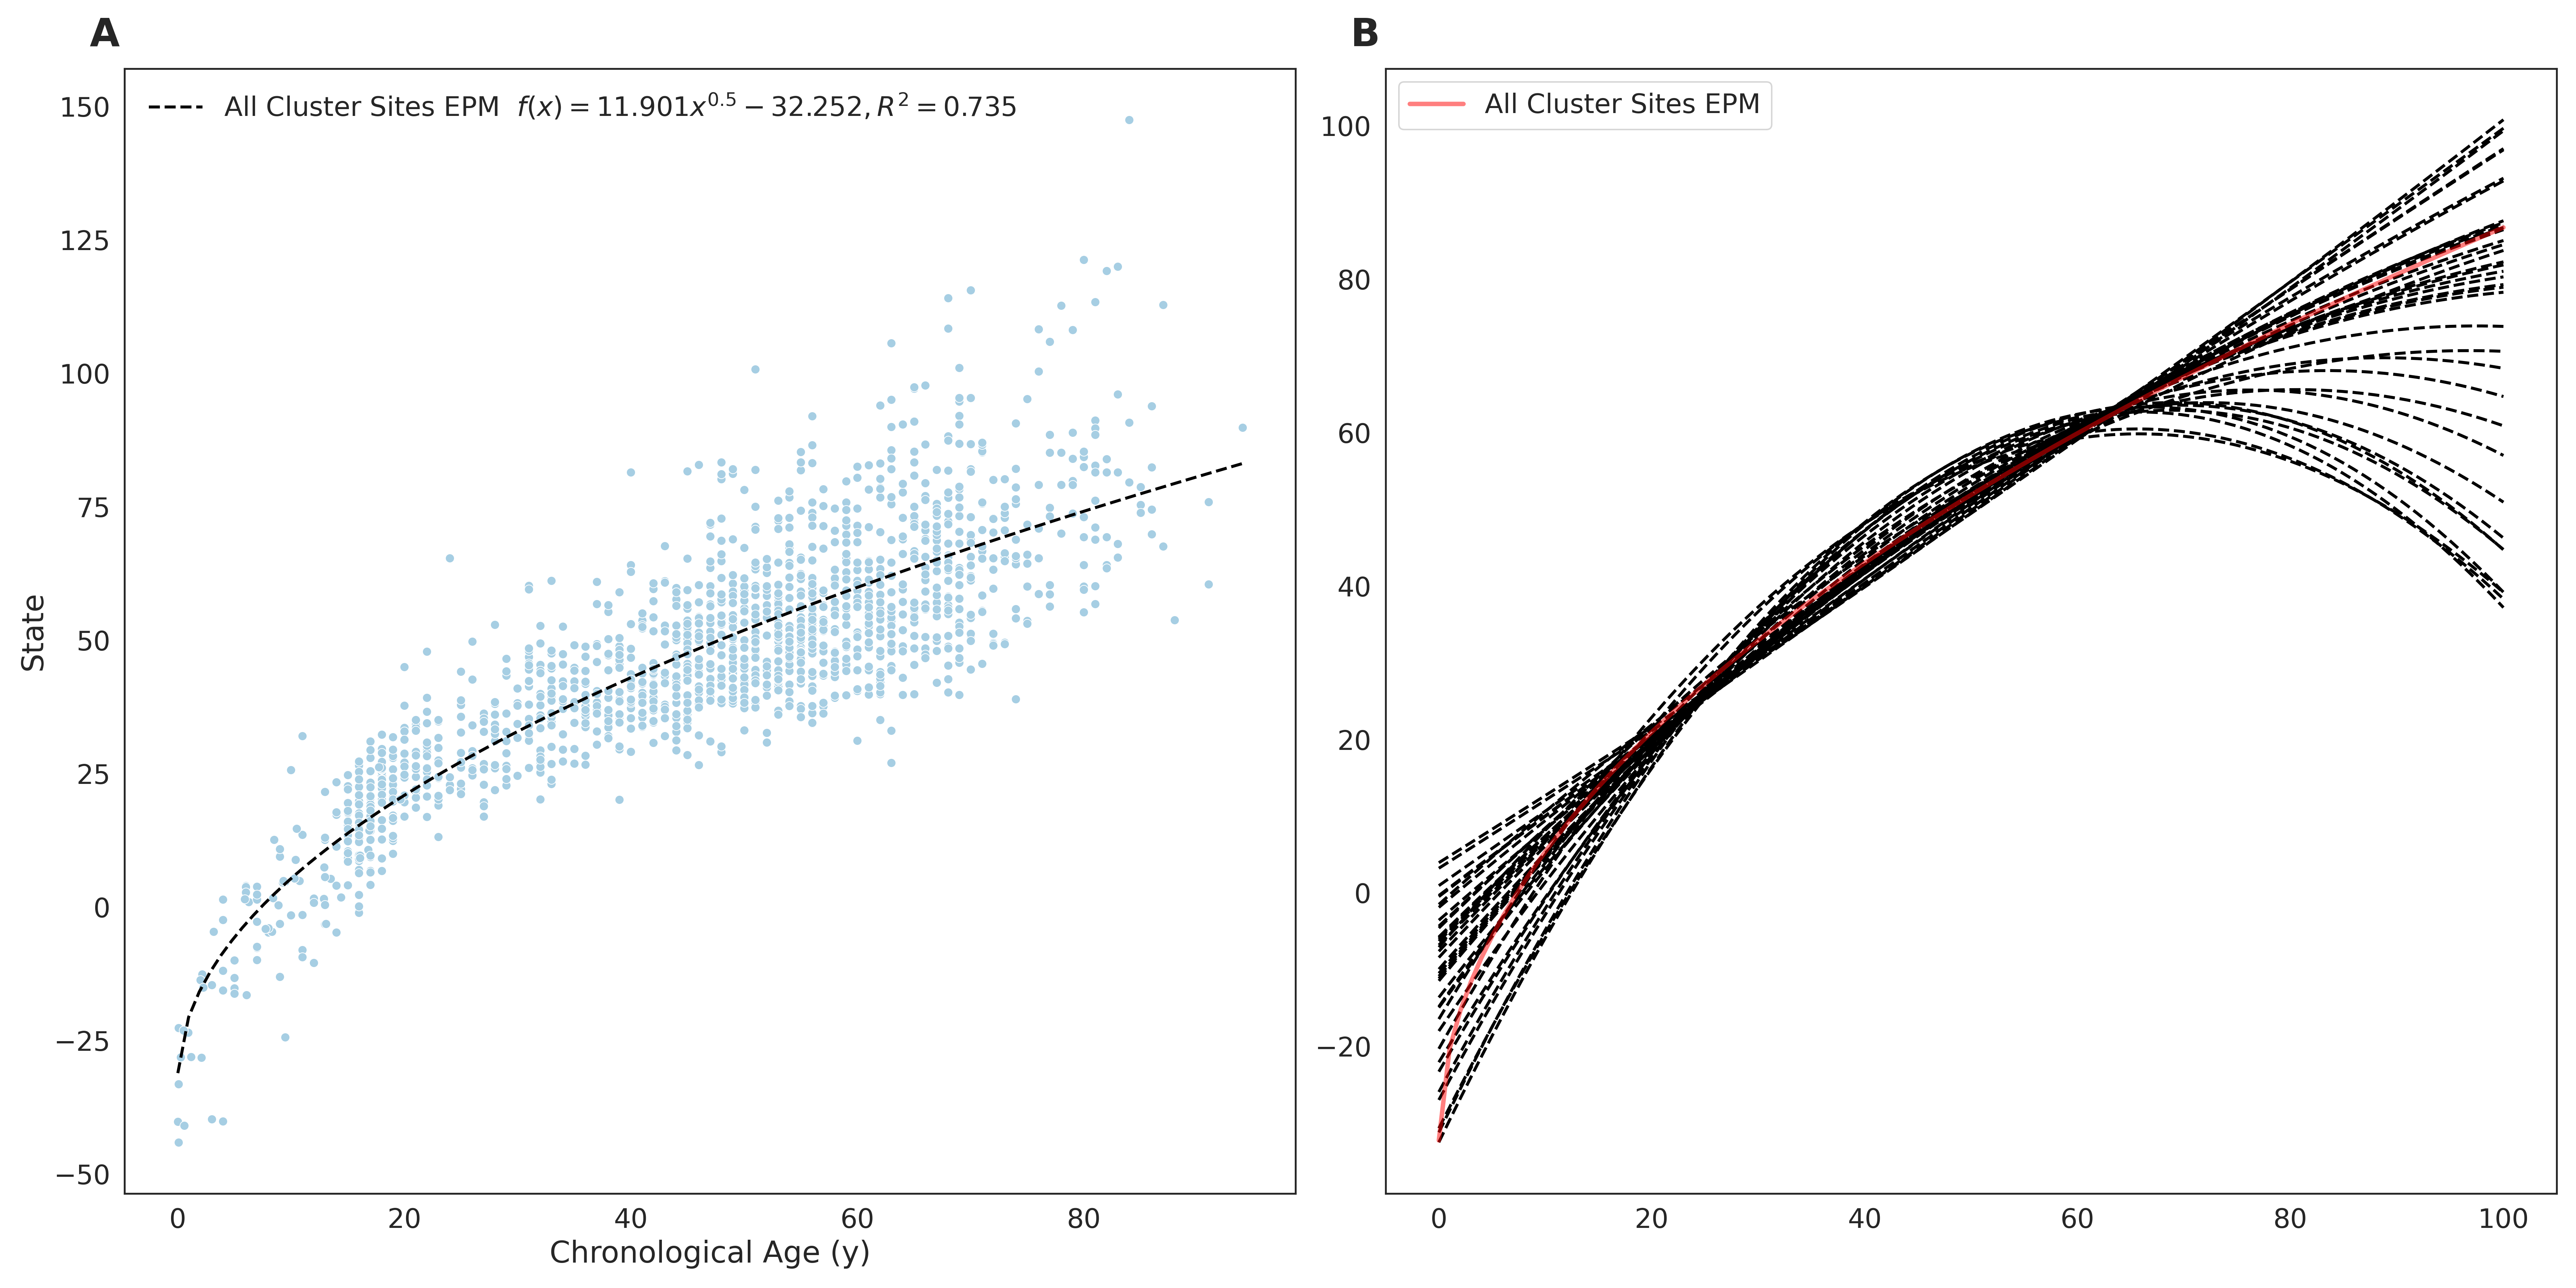
\includegraphics[scale=.25]{Figures/Figure3.png}
    \footnotesize
    \caption*{\small \textbf{Figure3:} \textbf{A} EPM model fit with 3832 methylation sites with a MAE below 0.025. 
                    \textbf{B} The fit trend line for EPM clusters with more than 10 sites and an $R^2 \geq 0.4$.}
    \end{figure}
\end{center}

\begin{raggedleft}
\begin{figure}

\includegraphics[scale=.18]{Figures/Figure4.png}
\footnotesize
\caption*{\small \textbf{Figure4: }Whole blood tissue validation \textbf{A} EPM, \textbf{B} cluster penalized 
regression and \textbf{C} full penalized regression models.}
\end{figure}
\end{raggedleft}

\begin{center}
    \begin{figure}
    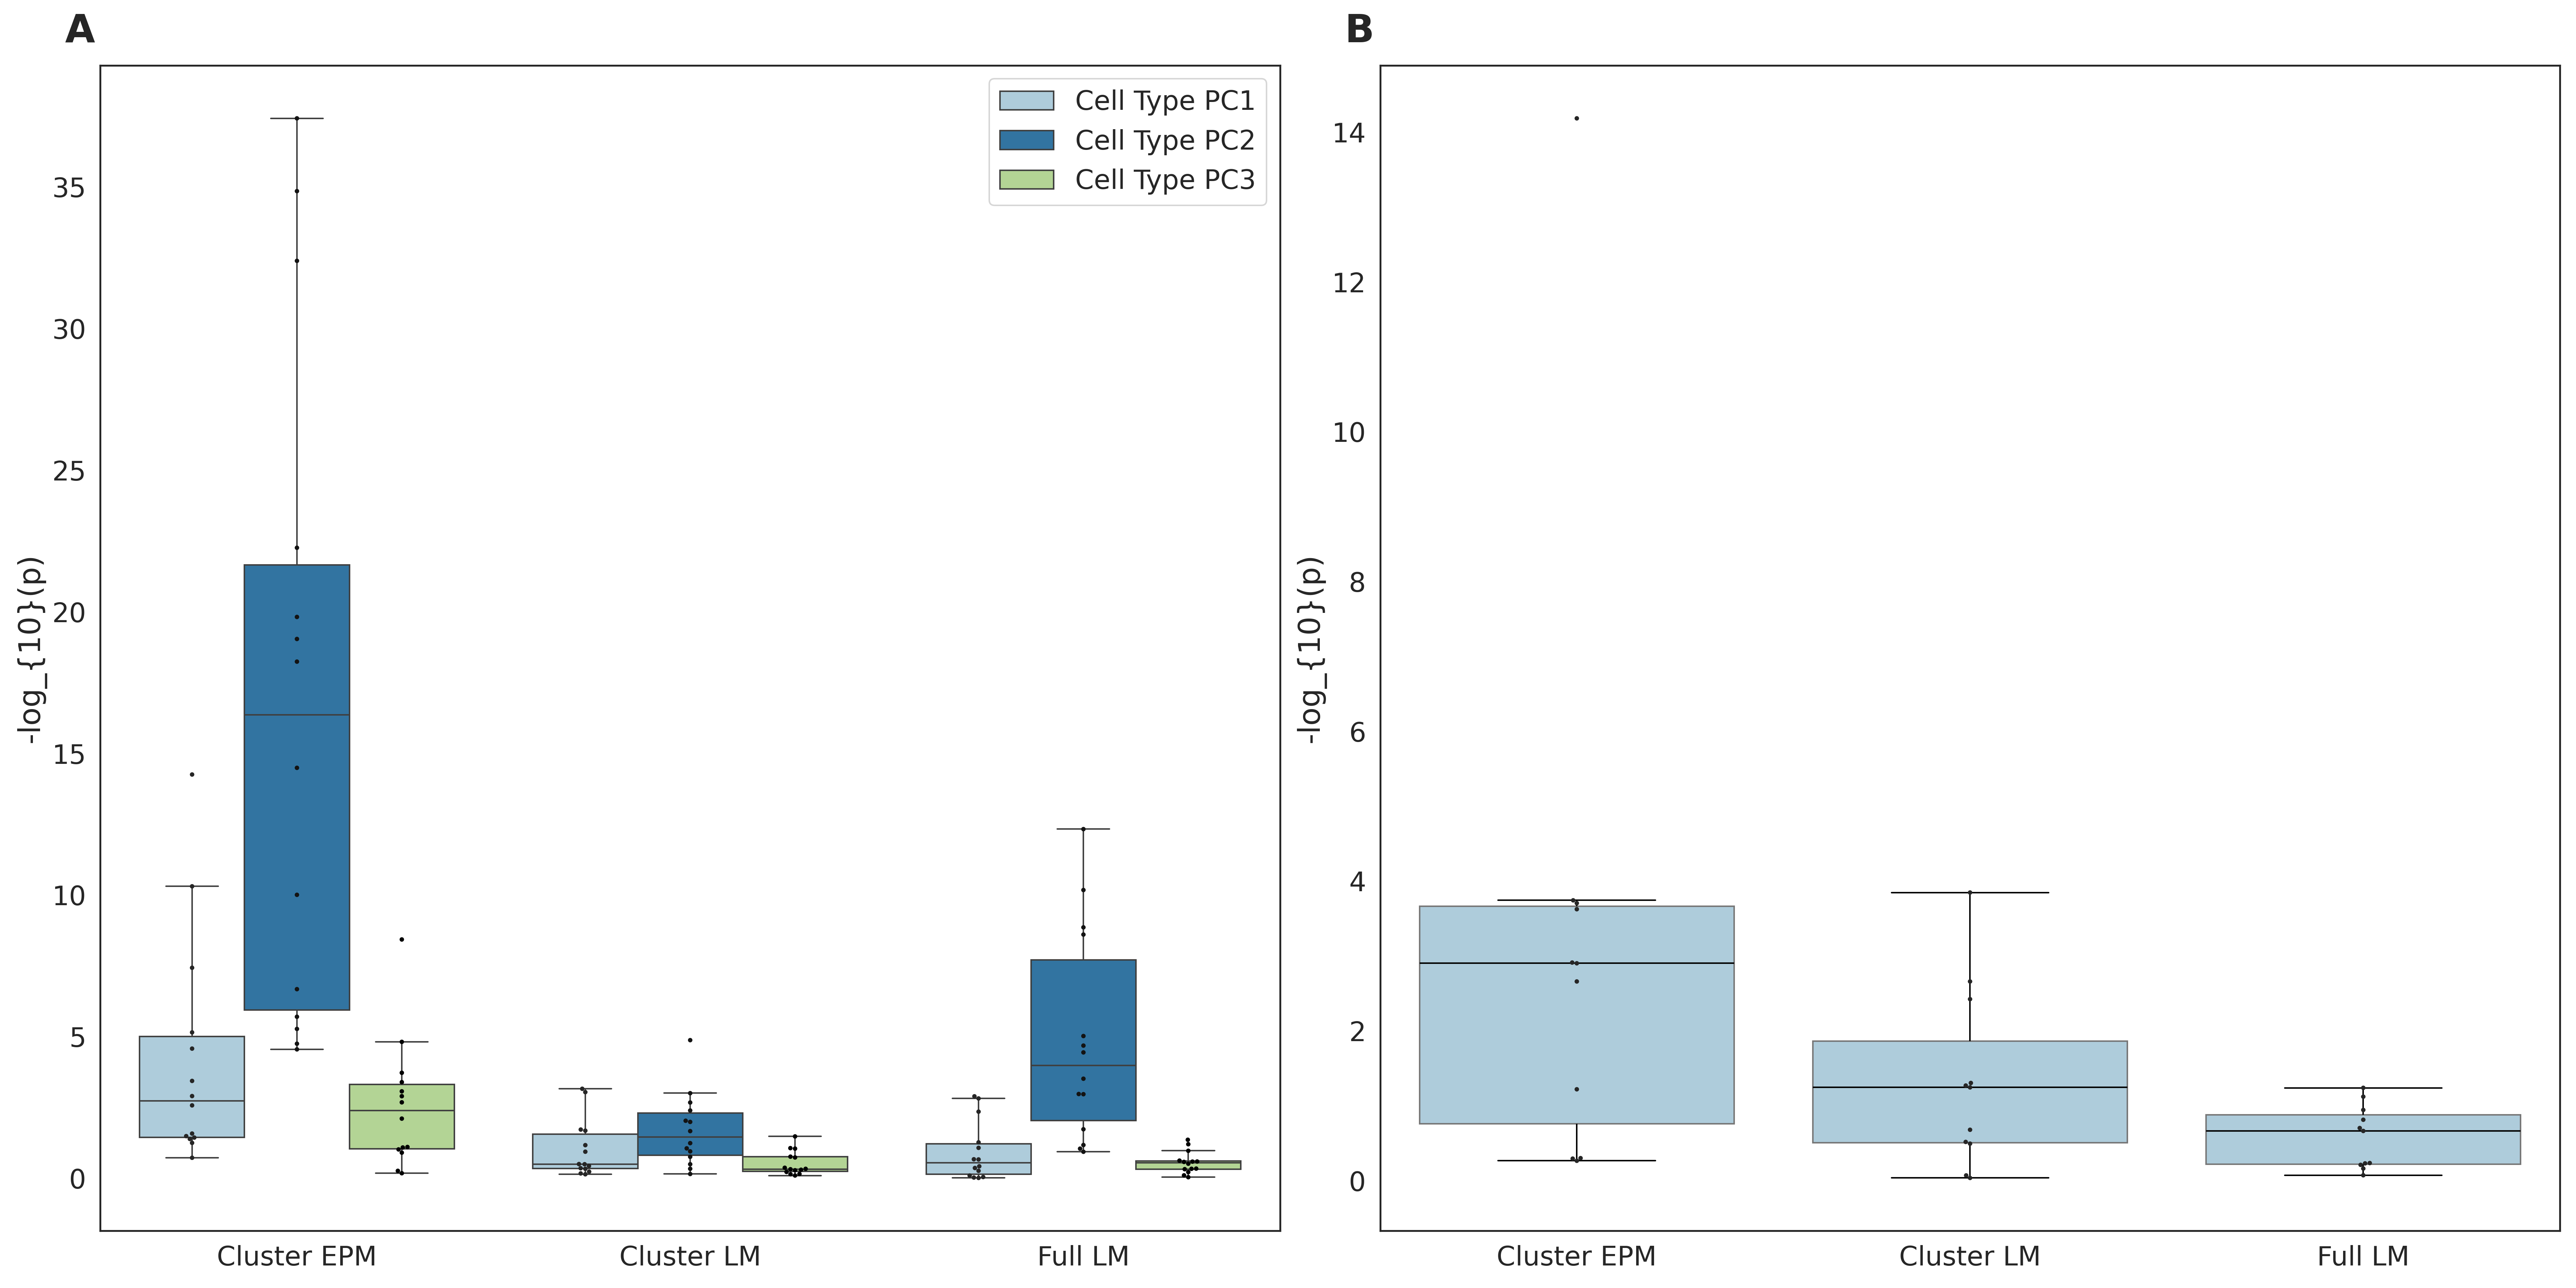
\includegraphics[scale=.25]{Figures/Figure5.png}
    \footnotesize
    \caption*{\small \textbf{Figure5: }\textbf{A} Cell type principal component and \textbf{B} predicted sex 
    regression coefficient p-values.
    }
    \end{figure}
\end{center}

\begin{raggedleft}
\begin{figure}
\includegraphics[scale=.15]{Figures/SFigure1.png}    
\footnotesize
\caption*{\small \textbf{S.Figure1: }Universal blood EPM and regression models. \textbf{A - C} Train, testing, and 
validation EPM model. \textbf{D-E}  Train, testing, and validation cluster penalized regression model. 
\textbf{G-J} Train, testing, and validation full penalized regression model.}
\end{figure}
\end{raggedleft}

\begin{center}
    \begin{figure}
    \includegraphics[scale=.25]{Figures/SFigure2.png}
    \footnotesize
    \caption*{\small \textbf{S.Figure2: }PBB EPM and regression models. \textbf{A - B} Train and testing EPM model. 
    \textbf{C-D} Train and testing penalized regression model.}
    \end{figure}
\end{center}

\end{document}